\chapter{Analýza}
%% TODO: zde napsat prehledovy text o tom, co vsechno tato kapitola obsahuje

\section{Problematika návrhu software}
Při návrhu software se uplatňují nejrůznější přístupy, vzory, pravidla. Cílem této sekce je podat rychlý přehled o používaných návrhových konceptech, aspektech návrhu software a objektově orientovaném návrhu. U některých aspektů uvažujeme možnost jejich podpory pomocí vhodného nástroje. Mnoho z uvedených pojmů a postupů je dále použito při návrhu nástroje, jehož vytvoření je jedním z cílů této práce.

\subsection{Koncepty používané při návrhu software}
Existující koncepty návrhu software poskytují vývojářům základ, z~něhož lze odvodit a aplikovat další sofistikované metody \cite{wiki:software_design}. Většinou se jedná o různé pohledy na způsob dekompozice systému na části realizovatelné v konkrétním programovacím jazyce. Postupem času se vyvinula celá množina konceptů návrhu software \cite{swengineeringconcepts}. Uveďme alespoň některé:

\paragraph{Abstrakce (Abstraction)} Abstrakce je proces nebo výsledek zobecnění a redukce informačního obsahu konceptu nebo pozorovatelného jevu. Typicky ponecháváme pouze informaci, která je relevantní pro konkrétní účel nebo záměr.

\paragraph{Postupné zjemňování (Refinement)} Postupné zjemňování/zpřesňování představuje proces tvorby\footnote{Tento koncept byl použit i pro tvorbu této práce. Nejprve byla provedena dekompozice tématu na základní bloky (specifikace, analýza, návrh, \ldots) a poté byly \uv{rekurzivním sestupem} realizované další sekce, podsekce a nakonec i elementární součásti práce (odstavce a věty).}. Je vytvářena hierarchie dekompozicí makroskopických příkazů funkce po krocích, dokud nejsou dosaženy elementární příkazy programovacího jazyka. V každém kroku je dekomponována jedna nebo více instrukcí daného programu do detailnějších instrukcí. Abstrakce a zjemňování jsou vzájemně komplementární oblasti.

\paragraph{Modularita (Modularity)} Systém je rozdělen do samostatných komponent nazvaných moduly (popsáno dále v podsekci \ref{analysis-sw_design_aspects}).

\paragraph{Architektura (Software Architecture)} Tento pojem odkazuje na celkovou strukturu softwarového systému a způsoby, kterými tato struktura zajišťuje konceptuální ucelenost systému.

\paragraph{Hierarchie řízení (Control Hierarchy)} Struktura programu, která reprezentuje organizaci programových komponent a určuje hierarchii řízení. Tato struktura však nedefinuje přesné pořadí operací.

\paragraph{Strukturální dělení (Structural Partitioning)} Struktura programu může být definována jak v horizontálním, tak vertikálním smyslu. Horizontální dělení představuje samostatné větve hierarchie modulů pro hlavní funkčnosti programu. Vertikální dělení slouží k distribuci řízení a průběhu zpracování do jednotlivých úrovní (vysokoúrovňové rutiny a nízkoúrovňové operace).

\paragraph{Struktura dat (Data Structure)} Logická reprezentace vztahů mezi jednotlivými datovými elementy.

\paragraph{Softwarová procedura (Software Procedure)} Koncept \emph{softwarové procedury} se zaměřuje na průběh zpracovávání každého jednotlivého modulu. Narozdíl od konceptu \emph{hierarchie řízení}, který se zabývá pouze vztahy (která komponenta je řízena kterou komponentou), se zaměřuje na návrh přesné posloupnosti kroků, které modul provádí.

\paragraph{Zapouzdření (Information Hiding)} Moduly by měly být navrhovány tak, aby informace v nich obsažená byla nedostupná modulům, které tuto informaci nepotřebují.

\subsection{Aspekty návrhu software}
\label{analysis-sw_design_aspects}
Při návrhu software musíme vzít v~potaz velké množství aspektů \cite{wiki:software_design}. Důležitost přikladaná jednotlivým aspektům je odvozena od účelu, za nímž je software realizován. Pro některé systémy může být klíčové rozšiřitelnost, pro jiné stabilita. Mezi základní aspekty patří:

\begin{itemize}
\item \emph{kompatibilita (compatibility)},
\item \emph{rozšiřitelnost (extensibility)},
\item \emph{zotavení se z~chyb (fault-tolerance/graceful degradation)} \cite{wiki:fault-tolerance},
\item \emph{udržovatelnost (maintainability)},
\item \emph{modularita (modularity)},
\item \emph{balení (packaging)},
\item \emph{spolehlivost (reliability)},
\item \emph{znovupoužitelnost (reusability)},
\item \emph{stabilita (robustness)},
\item \emph{bezpečnost (security)},
\item \emph{použitelnost (usability)}.
\end{itemize}

Zatímco některé aspekty jsou pro tuto práci zcela nepodstatné (dobrým příkladem budiž \emph{balení}, které se zabývá způsobem dodávky software a podporných materiálů), jiné je možné podpořit pomocí vhodného nástroje. Pojďme se nyní podívat na aspekty, jejichž podpora možná je:

\paragraph{Rozšiřitelnost} Tato vlastnost znamená praktický důsledek, kdy nové funkčnosti mohou být do existujícího systému přidány bez majoritních změn ve \emph{výchozí architektuře}. Pokud by bylo možné určit pravidla, která určují základní architekturu a která je možné vynutit, bylo by možné při rozšiřování systému tato pravidla opět aplikovat, což by vedlo k~dodržení výchozí architektury.

\paragraph{Udržovatelnost} Klíčovou charakteristikou \emph{udržovatelnosti} je možnost obnovit stav systému v~rozumném čase. Příkladem mohou být aktualizace virové báze antivirových programů. Jiným příkladem může být instalace bezpečnostních aktualizací. Tuto vlastnost nelze podpořit zcela přímo, je však důsledkem ostatních vlastností (zejména \emph{rozšiřitelnost} a \emph{modularita}).

\paragraph{Modularita} \emph{Modularita} znamená, že výsledný systém sestává z~dobře definovaných a nezávislých komponent. To vede k~lepší \emph{udržovatelnosti}. Komponenty mohou být v~takovém případě vyvíjeny a testovány izolovaně předtím než jsou integrovány do výsledného požadovaného softwarového systému. Navíc získáme dobrou možnost dělby práce v~rámci vývojového týmu pracujícího na softwarovém projektu.

\paragraph{Znovupoužitelnost} Je důležité, aby bylo možné přidávat nové vlastnosti (features) systému a provádět modifikace s~pouze omezenou nebo žádnou modifikací existujících komponent (možnost použít komponenty znovu pro jiné případy užití).

\subsection{Objektově orientovaný návrh software}
Základním vstupem pro objektově orientovaný návrh bývá (mimo jiné) \emph{konceptuální model}, případně seznam \emph{případů užití} systému. To jsou výsledky předešlé fáze analýzy. Na základě těchto informací je poté zpravidla sestavován návrh systému, který pracuje nad dříve definovanými doménovými objekty.

Klíčovými pojmy při objektově orientovném návrhu jsou \cite{wiki:oop_design}:

\paragraph{Objekt/třída}  Objekt/třída představují těsné propojení mezi datovými strukturami a metodami/funkcemi, které nad těmito daty pracují. Každý objekt by měl sloužit samostatné funkci. Je definován svými atributy/vlastnostmi, tím co je a tím co může dělat.
\paragraph{Zapouzdření} Zapouzdření je schopnost chránit některé součásti objektu před externími entitami. To je zpravidla realizováno klíčovými slovy implementujícího programovacího jazyka, která umožňují deklarovat proměnnou jako privátní nebo chráněnou uvnitř vlastnické třídy.
\paragraph{Dědičnost} Dědičnost umožňuje nové třídě rozšířit nebo i přepsat funkcionalitu jiné třídy. Výsledná podtřída má kompletní část, která je derivována z nadtřídy a navíc své vlastní funkce a data.
\paragraph{Rozhraní} Rozhraní představuje možnost odložení implementace metod. Je možné definovat signatury funkcí nebo metod, aniž by bylo nutné tyto metody implementovat.
\paragraph{Polymorfismus} Polymorfismus nám umožňuje nahradit objekt jeho podobjektem (instancí podtřídy). Proměnná tedy může obsahovat buď objekt nebo kterýkoliv jeho podobjekt.

Při vlastním návrhu systému se používají principy objektového návrhu (popsáno dále v sekci \ref{analysis-oop_design_principles}) a návrhové vzory. Pro realizaci objektových systému se potom používají nejrůznější frameworky a knihovny.

\section{Analýza principů objektového návrhu}
\label{analysis-oop_design_principles}

Principy objektového nárhu reprezentují množinu pokynů, které nám pomáhají vyhnout se špatnému návrhu \cite{oop_design_principles}. Špatný návrh vykazuje zejména následující vlastnosti \cite{oop_design_principles_and_patterns}:

\begin{itemize}
\item \emph{Rigidity} -- je obtížné provést změnu v systému protože každá změna ovlivňuje příliš mnoho dalších částí systému,
\item \emph{Fragility} -- pokud provedete změnu, mohou přestat fungovat části systému u nichž se to nečeká,
\item \emph{Immobility} -- je obtížné znovupoužití části systému v jiné aplikaci, protože tato část nemůže být \uv{vymotána} z aktuální aplikace.
\end{itemize}

Autor výše zmíněného článku (\cite{oop_design_principles_and_patterns}) cituje zajímavé návrhové principy. Například \emph{Open Closed Principle}, který vyžaduje, aby se existující třídy a řešení nemodifikovaly, ale rozšiřovaly. Dalším principem je \emph{Liskov's substitution principle}, který vymezuje pravidla pro dědění tak, aby instance podtřídy mohla bezpečně vystupovat na místě své nadtřídy\footnote{Ve článku je rozebráno, jaké operace bychom neměli provádět v oddědědné třídě -- je totiž možné změnit chování odděděné třídy tak, že již nemůže bezpečně vystupovat na místě svého předka.}.

Důležité je srovnání \emph{návrhových principů} s \emph{návrhovými vzory}. Toto srovnání podává článek \cite{612257}. Zatímco aplikace návrhového vzoru představuje znovupoužití \uv{úspěšného} návrhu, princip představuje spíše obecně platné pravidlo, jehož dodržováním během návrhu bychom měli získat návrh přijatelné kvality. V případě přesného stanovení potřebných principů by bylo možné provádět automatizovný systematický návrh (což není, vzhledem k mnoha aspektům popisovaným v článku, dobře možné).

\subsection{Analyzované principy}
Na základě požadavků specifikovaných sekci \ref{requirements-principle_analysis} se budeme postupně zabývat principy \emph{low coupling}, \emph{high cohesion} a \emph{Law of Demeter}. Jedná se o~principy, které se týkají strukturální kvality kódu.

Ukázkové návrhové principy a vztahy mezi nimi jsou znázorněny na obrázku \ref{analyzed_principles}. Poznamenejme, že \emph{Law of Demeter} (dále budeme používat zkratku \emph{LoD}) je konkretizací požadavků na \emph{nízkou závislost} (\emph{low coupling}) mezi moduly.

\begin{figure}[h!]
  \centering
  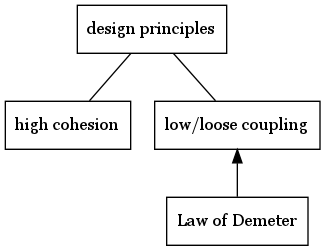
\includegraphics[width=0.5\textwidth]{./graphs/oop_design_principles.png}
  \caption{Znázornění analyzovaných návrhových principů.\label{analyzed_principles}}
\end{figure}

\subsubsection{Low coupling/dependency (nízká závislost/vazba)}

%% * [[Measuring coupling and cohesion in object-oriented systems|http://www.isys.uni-klu.ac.at/PDF/1995-0043-MHBM.pdf]]
%% * [[Defining and validating high-level design metrics|http://citeseerx.ist.psu.edu/viewdoc/download?doi=10.1.1.31.4744&rep=rep1&type=pdf]]
%% * [[Bieman, J.M.; Byung-Kyoo Kang; , "Measuring design-level cohesion," Software Engineering, IEEE Transactions on , vol.24, no.2, pp.111-124, Feb 1998|http://ieeexplore.ieee.org/stamp/stamp.jsp?tp=&arnumber=666825&isnumber=14664]]

Závislost/vazba (coupling/dependency) mezi moduly softwarového projektu určuje, do jaké míry se jeden modul spoléhá na každý z~ostatních modulů \cite{wiki:coupling}. Zatímco některé moduly spolu vůbec nekomunikují (nemají žádnou závislost), jiné se spoléhají nejen na rozhraní ostatních modulů, ale mnohdy i na jejich vnitřní fungování, způsob reprezentace dat, časování atd. Důsledkem vyšší závislosti je potom nutnost rozsáhlých úprav v~mnoha modulech i při úpravě naprostých drobností v~jednom konkrétním modulu.

Proto je důležitou návrhovou zásadou snaha snížit závislost modulů na minimum. Je zřejmé, že závislost mezi moduly vždy existuje (jinak by neměl modulární návrh smysl). Proto nelze striktně říci, do jaké míry smí/nesmí být moduly na sobě závislé.

V~\cite{wiki:coupling} a \cite{STVR:STVR162} (podrobnější a formálnější definice) je podáván přehled úrovní závislosti jednoho modulu na druhém. Následující zjednodušený seznam úrovní závislostí je seřazen od nejvyšší fromy závislosti po nejnižší:

\paragraph{Content coupling (nejvyšší forma závislosti)} Jeden modul modifikuje jiný modul nebo se spoléhá na vnitřní fungování jiného modulu (např. přístup k~lokálním datům jiného modulu). V~důsledku platí, že změní-li se způsob, kterým tento druhý modul produkuje data (umístění, typ, časování), povede to zcela jiste ke změnám v~závislém modulu.

\paragraph{Common coupling} Dva moduly sdílí stejná globální data (např. globální proměnnou), změna sdíleného globálního zdroje implikuje změny všech modulů, které je používají.

\paragraph{External coupling} Dva moduly sdílí externě definovaný (standardizovaný) datový formát, komunikační protokol nebo rozhraní zařízení.

\paragraph{Control coupling} Jeden modul kontroluje tok druhého tím, že mu posílá informaci o~tom, co má konat (např. předání \uv{to-do} příznaku).

\paragraph{Stamp data coupling} Jeden modul předává druhému modulu složenou datovou strukturu jako parametr. Ten ji používá pouze pro výpočty (nikoliv pro rozhodování řízení toku programu).

\paragraph{Scalar data coupling} Moduly sdílí data pomocí parametrů. Každý parametr je elementární datový typ a jedná se o~jediná data, která jsou sdílená (např. předávání celočíselné hodnoty funkci, která spočítá jeho druhou mocninu). Modul, kterému jsou předávány parametry, jich používá pouze k~výpočtu hodnoty a nikoliv pro rozhodování řízení toku programu.

\paragraph{Message coupling (nejnižší forma závislosti)} Moduly jsou komunikují pouze pomocí posílání zpráv (message passing). Jedná se o~nejnižší úroveň závislosti. Moduly o~sobě navzájem nemusí mít žádnou znalost. Moduly nepoužívají vzájemně žádné předávání parametrů, nemají žádné sdílené reference na objekty nebo globální data.

\paragraph{Independent coupling/No coupling} Mezi moduly není žádná závislost. Moduly spolu vůbec nekomunikují a nejsou zde žádné sdílené reference na proměnné nebo reference na externí data sdílená mezi moduly.

\vspace{0.5cm}

\paragraph{Subclass coupling} Pro objektově orientovaný návrh můžeme navíc uvažovat závislost typu \emph{Subclass coupling}, která popisuje vztah mezi třídou a její rodičovskou třídou. Dětská třída má závislost na rodičovské, rodičovská však žádnou závislost vzhledem k dětské třídě nemá.

\vspace{1.0cm}

Cílem návrhu je snižovat co nejvíce míru závislosti modulů. Protože se ale jedná o~kvantitativní záležitost, nejsme schopni určit zcela přesná pravidla, která musí platit nebo která lze vynutit. U~některých typů programů může být akceptovatelý i \emph{content coupling} z~výkonnostních důvodů\footnote{Nízká vazba implikuje téměř vždy snížení výkonu z~důvodu nutnosti dalších mechanismů, které zprostředkovávájí komunikaci mezi moduly (např. \emph{message passing} mechanismus).}, naopak u~jiných systémů může být nízká vazba (\emph{message coupling}) dána již návrhem (např. CORBA, web services, atd.).

\subsubsection{High cohesion (vysoká koheze/soudržnost)}
Pojmem \emph{koheze} je označována míra, jak silně související/příbuzná je funkcionalita vyjádřená modulem programu \cite{wiki:cohesion}. Existují různé přístupy k měření této metriky, od kvalitativních, vyjadřujících se pomocí slovních ohodnocení, po kvantitativní, vyjadřující míru soudržnosti kódu pomocí čísel.

Moduly s vysokou kohezí jsou zpravidla preferovány, protože jejich vlastnosti implikují \uv{dobré} vlastnosti návrhu včetně stability, spolehlivosti, znovupoužitelnosti a srozumitelnosti, zatímco moduly s nízkou kohezí je obtížné udržovat a testovat.

Ke snížení koheze dochází když:
\begin{itemize}
\item funkcionalita vyjádřená třídou, ke které přistupujeme pomocí metod, nemá mnoho společného
\item metody provádějí velké množství rozdílných aktivit často nad rozsáhlými nebo nesouvisejícími daty
\end{itemize}

Nevýhodou nízké koheze je:
\begin{itemize}
\item obtížnější porozumění modulům,
\item obtížnější údržbu systému -- logické změny v řešené doméně ovlivňují více modulů a také proto, že změny v jednom modulu vyžadují změny v modulu jiném,
\item otížnější znovupoužití modulu -- většina aplikací nepotřebuje náhodnou množinu operací, kterou modul poskytuje.
\end{itemize}

Kohezi můžeme uvažovat na různých úrovních. Jako úroveň můžeme zvolit např. metodu, třídu, balíček, modul nebo projekt. Program může mít vysokou kohezi na úrovni tříd (metody jsou dobře seskupené ve třídách podle funkcionality a pracují nad shodnými daty), zatímco na úrovni balíčků může vykazovat nižší kohezi (třídy v rámci balíčku spolu logicky nesouvisí).

Problematikou soudržnosti programových modulů se zabývá článek \cite{Kang:1996:DCM:872750.873361}, který představuje dvě různé metriky používané k jejímu měření.

Článek \cite{ISI:000079726000029} uvádí dělení koheze podle tzv. SMC\footnote{Podle původních autorů Stevens, Myers a Constantine.} Cohesion. Míra koheze je vyjádřena na základě typu asociace mezi procesními elementy (seřazeno od nejnižší úrovně koheze po nejvyšší):

\paragraph{Coincidental association} Neexistuje souvislost mezi elementy provádějícími zpracování.

\paragraph{Logical association} Oba elementy provádějící zpracování patří do stejné logické třídy příbuzných funkcí.

\paragraph{Temporal association} Každý výskyt obou elementů provadějících zpracování je v~tom samém omezeném časovém období při provádění programu.

\paragraph{Procedural association} Oba elementy provádějící zpracování jsou elementy stejné procedurální jednotky, která je iterativním nebo rozhodovacím procesem.

\paragraph{Communicational association} Oba elementy provádějící zpracování pracují nad stejnou množinou vstupních dat a/nebo produkují stejná výstupní data.

\paragraph{Sequential association} Výstupní data jednoho elementu jsou vstupními daty pro druhý element.

\paragraph{Functional association} Oba elementy jsou nezbytné pro provedení jedné funkce/operace.

\subsubsection{Law of Demeter}

% TODO: complete this section

%% Adaptive Object-Oriented Software The Demeter Method -- http://www.google.cz/url?sa=t&source=web&cd=3&sqi=2&ved=0CCoQFjAC&url=http%3A%2F%2Fciteseerx.ist.psu.edu%2Fviewdoc%2Fdownload%3Fdoi%3D10.1.1.94.8349%26rep%3Drep1%26type%3Dpdf&rct=j&q=demeter%20software%20object%20oriented&ei=MeTOTPihHI7AswbpufiWCA&usg=AFQjCNHnRixmCYTZrJVPF2OCEcbooajq4A&cad=rja
%% The Law of Demeter Is Not A Dot Counting Exercise -- http://bit.ly/9tCObJ]] - pěkný popularizační článek na úvod
%% Object-oriented programming: an objective sense of style -- http://portal.acm.org/ft_gateway.cfm?id=62113&type=pdf&coll=GUIDE&dl=GUIDE&CFID=111192652&CFTOKEN=98650016
%% Formulations and benefits of the law of demeter -- http://portal.acm.org/citation.cfm?id=643603.643608
%% Demeter: Aspect-Oriented Software Development -- http://www.ccs.neu.edu/research/demeter/
%% A case for statically executable advice: checking the law of demeter with AspectJ -- http://portal.acm.org/citation.cfm?id=643603.643608

Existuje několik forem Demeterova zákona \cite{35588}, které jsou vhodné pro různé oblasti aplikace. Tyto typy jsou znázorněny na obrázku \ref{demeter_law_types}. V~\cite{35588} se též pojednává o~demeterově zákoně z~jiného úhlu -- uvažují se všechny možné třídy, které lze volat bez porušení tohto principu (tzv. preferred suppliers).

\begin{figure}[h!]
  \centering
  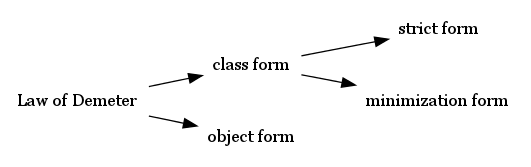
\includegraphics[width=0.7\textwidth]{./graphs/demeter_law_types.png}
  \caption{Formy návrhového principu LoD.\label{demeter_law_types}}
\end{figure}

Pro statickou analýzu lze použít \uv{class} formu Demeterova zákona.

% TODO: rozhodnout, kterou verzi Demeterova zákona použít

\emph{Zjednodušená verze \cite{wiki:lod}}

Method M of an object O~may only invoke the methods of the following kinds of objects:

\begin{itemize}
\item O~itself,
\item M's parameters,
\item any objects created instantiated within M,
\item O's direct component objects,
\item a global variable, accessible by O~in the scope of M.
\end{itemize}

\subsection{Ukázky kódu porušujícího některá z~pravidel}
% TODO: v rámci každého návrhového principu uvést příklad porušení tohoto principu (případně i příklad, který tento princip dodržuje)

\subsubsection{Porušení principu law of Demeter}

% TODO: find some better (real world) example of demeter law violation on the web
\lstset{
  basicstyle=\ttfamily,
  numbers=left,
  numberstyle=\tiny,
  commentstyle=\color{gray}\textit
}
\begin{lstlisting}[language=java]
  package violations;

  public class DemeterLawViolation {

    void method(MyClass obj, int val) {

      obj.getSomeInternalField().setValue(val);

      // hidden violation:
      InternalFieldDef internalField =
      obj.getSomeInternalField();
      internalField.setValue(val);

    }

  }
\end{lstlisting}

\section{Analýza problematiky v~jazyce Java}

V rámci této sekce se podíváme nejprve na to, z čeho se skládá softwarový systém realizovaný v programovacím jazyce Java. Ve druhé části je provedena rešerše existujících nástrojů pro zpracování zdrojových kódů programovacího jazyka Java do podoby vhodné pro vygenerování potřebné vnitřní struktury, která bude předmětem validace.

\subsection{Statický model programu v~Javě}
Vstupem pro validační systém budou zdrojové kódy existujícího Java projektu ve vhodné podobě. Jedná se vlastně o fyzický model programu. V případě Java projektu sestává tento model z nějaké množiny souborů, které obsahují data různých typů. První podsekce této sekce se zabývá typy souborů, které se mohou vyskytnout v projektu, ve druhé podsekci je potom rozebírán obsah a formát souborů programovacího jazyka Java.

Zastavme se ještě nad pojmem \emph{fyzický model} programu. Tento model je zpravidla výsledkem vhodné transformace (ať už automatizované nebo ruční) nějakého předešlého modelu (většinou UML model, textová specifikace atd.). S tímto modelem můžeme dále pracovat a provádět nad ním transformace. To je ostatně cílem různých nástrojů pro refaktoring a automatizované zvyšování kvality kódu. Konkrétně refactoring je příkladem endogenní horizontální transformace (zdrojový i cílový metamodel je shodný a úroveň abstrakce zůstává nezměněna) \cite{Mens05ataxonomy}.

\subsubsection{Struktura softwarového projektu v~Javě}
Existuje velké množství způsobů, kterými jsou organizovány softwarové projekty. Téměř každé Java IDE má navíc svůj vlastní formát, ve kterém ukládá metadata o projektu. Přesto všechny tyto projekty zahrnují stejnou podmnožinu konkrétních zdrojových souborů, z nichž se skládá vlastní softwarový projekt. Podívejme se, jaké soubory můžeme nalézt v běžném java projektu:

\begin{itemize}
\item soubory \verb+*.java+ -- soubory se zdrojovými kódy v jazyce Java, tyto soubory představují z hlediska gramatiky jazyka Java kořenový element \emph{CompilationUnit} (o něm bude dále pojednáno v podsekci \ref{analysis-java_grammar_elements}),
\item binární součásti projektu -- soubory \verb+*.jar+ a \verb+*.class+, často se jedná o různé knihovny, zkompilované \verb+*.java+ soubory atd.
\item build scripty a konfigurační soubory sestavovacích nástrojů (\verb+build.xml+, \verb+pom.xml+, \ldots),
\item soubory zdrojů (resources, resource bundles) -- read-only data využívaná programem (ikony, lokalizační řetězce, atd.)
\item dokumentace (\verb+javadoc+, uživatelská příručka),
\item soubory gramatik pro parsery a \emph{compiler-compiler} systémy (např. pro \verb+lex+, \verb+flex+, \verb+javacc+, \verb+antlr+),
\item šablony (typické třeba pro webové projekty, \verb+*.xhtml+ a jiné přípony),
\item konfigurační soubory (zpravidla \verb+*.xml+ soubory, často odkazují konkrétní třídy progamovacího jazyka Java),
\item jiné soubory
\end{itemize}

Pro potřeby této práce jsou podstané v zásadě pouze soubory obsahující zdrojový kód -- soubory \verb+*.java+. Při analýze nebudeme program spouštět nebo uvažovat jeho dynamické chování (běh). Bude se jednat o analýzu statického stavu programu (analýza struktury). Práce bude probíhat nad definicemi tříd, nikoliv nad jejich instancemi v~paměti JVM. Nejsou tedy uvažovány všechny možné běhové instance programu (všechny možné stavy objektů v~paměti virtuálního stroje).

Projekt může záviset na velkém množství dalších tříd, které nejsou součástí zdrojových kódů projektu. Tyto třídy zpracovávat nebudeme. Jedná se například o:

\begin{itemize}
\item knihovny třetích stran,
\item standardní knihovnu jazyka Java (i.e. Java 2 Platform SE 5.0 API pro Javu verze 5),
\item podprojekty a části projektu, které analyzovat nechceme, nepotřebujeme nebo z~nějakého důvodu nemůžeme.
\end{itemize}

Některé z těchto tříd budou povolenými závislostmi pro všechny třídy projektu (např. všechny třídy projektu mohou záviset na standardních knihovnách jazyka Java), jiné budou naopak povolené jen pro určité oblasti projektu (budeme chtít, aby rozhraní pro přístup k databázi využívaly pouze objekty DAO vrstvy).

\subsubsection{Syntaktické elementy programovacího jazyka Java}
\label{analysis-java_grammar_elements}

% TODO: Budeme pracovat nad gramatikou jazyka Java 1.5. Java verze 6 se liší pouze úpravou standardních API poskytovaných platformou Java. Jazyk jako takový zůstává stejný.
Grafické znázornění základních syntaktických elementů, jejichž struktura a názvy jsou převzaty z~\cite{Gosling:2005:JLS:1036643}, je na obrázku \ref{toplevel_elements}.

\begin{figure}[h!]
  \centering
  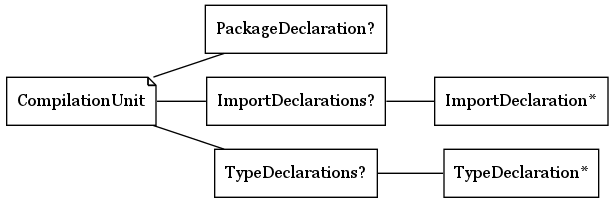
\includegraphics[width=0.85\textwidth]{./graphs/java_top_elements.png}
  \caption{Struktura základních syntaktických elementů programovacího jazyka Java.\label{toplevel_elements}}
\end{figure}

Pro analýzu založenou na vyhledávání závislostí mezi třídami pro nás bude nejdůležitější syntaktický element \emph{TypeDeclaration}. Tento neterminální symbol se dále přepisuje na symboly uvedené na obrázku \ref{type_declaration_options}.

\begin{figure}[h!]
  \centering
  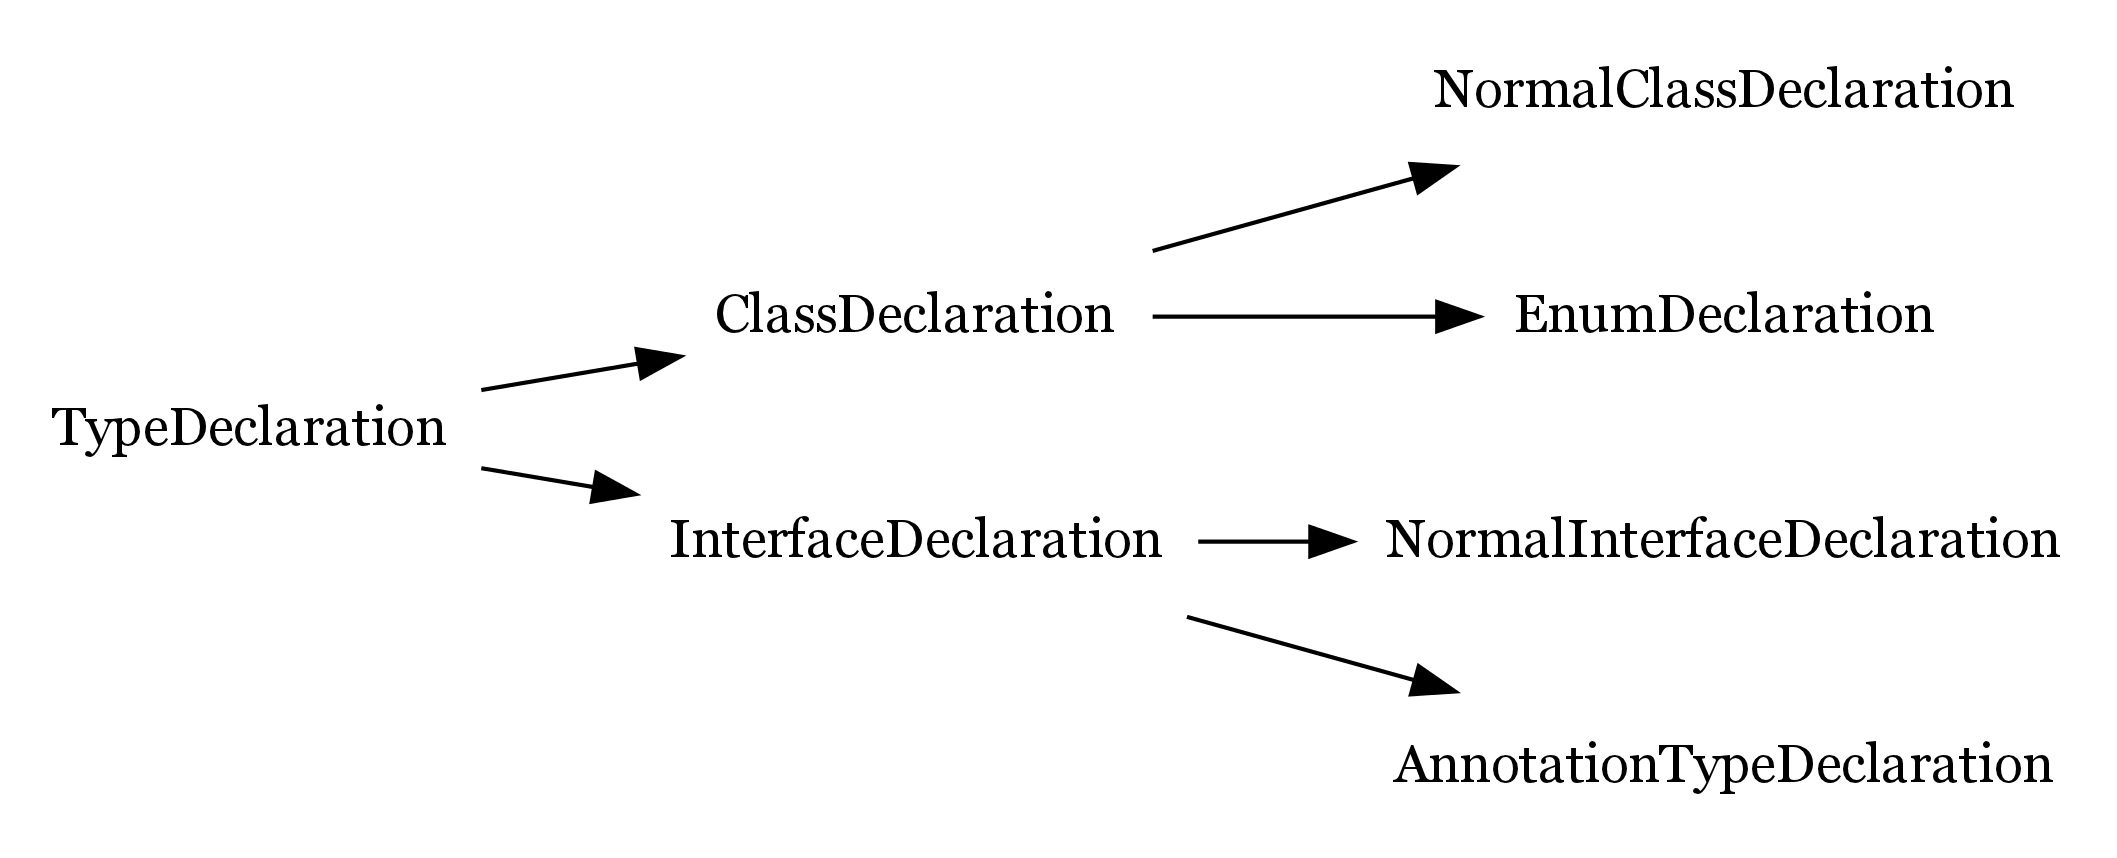
\includegraphics[width=\textwidth]{./graphs/toplevel_types.png}
  \caption{Rozklad elementu TypeDeclaration.\label{type_declaration_options}}
\end{figure}

\subsection{Zpracovávání zdrojových kódů v~jazyce Java}
Protože navrhované ověřované principy přesahují rámec jedné kompilační jednotky, je nutné provést vhodné předzpracování zrojových kódů tak, aby bylo možné analyzovat vztahy částí kódu i mezi jednotlivými kompilačními jednotkami.

V principu to znamená provést podobnou množinu operací, jakou provádí první kompilátor jazyka Java při kompilaci \cite{hackers_guide_to_javac}. Ten nejprve načte všechny \verb+*.java+ soubory a namapuje sekvence tokenů na uzly AST stromu. Následně vloží všechny nalezené symboly do tabulky symbolů (např. jména datových typů, proměnných atd.). Provede zpracování anotací nalezených v kompilačních jednotkách. Ve fázi \emph{attribute} jsou provedeny operace jako rozlišení jmen, kontrola datových typů a zjednodušení konstatních výrazů. Následuje kontrola datových toků v programu (pracuje na stromu získaném v předchozích krocích), která má za cíl určit např. nedostupné části zdrojového kódu (po příkazu return apod.). Předposlední fáze \emph{desugar} přepíše AST a zjednoduší některé výrazy používané jako \uv{syntaktický cukr} na jednodušší výrazy. Na závěr provede kompilátor vlastní vygenerování zdrojových kódů nebo class souborů. 

Pro provedení analýzy nám postačí zdrojové kódy zpracované do fáze \emph{attribute}. Jedná se o AST s rozlišenými jmény datových typů a proměnných. Nad těmito stromy můžeme dále pracovat.

Podívejme se nyní, jakými prostředky je možné tuto reprezentaci získat:

\subsubsection{Vlastní kód pro zpracovávání zdrojových kódů}
\begin{itemize}
\item vlastní hand-written lexikální a syntaktický analyzátor (zbytečně náročné)
\end{itemize}

\subsubsection{Použití compiler-compiler systému}
\begin{itemize}
\item parser vygenerovaný pomocí některého z~dostupných compiler-compiler systémů
\item existující gramatiky pro jazyk Java
\item generátory lexikálních analyzátorů a syntaktických parserů
\item generátory stromů
\end{itemize}

\begin{itemize}
\item tyto systémy na základě vstupní gramatiky vygenerují frontend pro překladač
\item lze specifikovat různé akce, které jsou navázány na události vyvolané v~průběhu syntaktické analýzy
\item \emph{JavaCC} \cite{parsertools:javacc}
  \begin{itemize}
  \item součástí je nástroj \emph{JJTree}, který je schopen vygenerovat AST pro další práci
  \end{itemize}
\item \emph{JastAdd} \cite {parsertools:jastadd}
\item \emph{ANTLR}
\end{itemize}

\subsubsection{Použití vhodné knihovny nebo existujícího programu}
\begin{itemize}
\item JavaParser \cite{parsertools:javaparser}
  \begin{itemize}
  \item projekt na GoogleHosting
  \item v~podstatě gramatika pro JJTree vytvářející strom tříd a objektů, který je možné procházet pomocí visitor patternu
  \end{itemize}
\item spoon \cite{parsertools:spoon}
\end{itemize}

\subsubsection{Použití prostředků poskytovaných platformou Java}
použití prostředků poskytovaných platformou Java 6 (Sun verze) \cite{source_code_analysis_corejavatechtips}
\begin{itemize}
\item \emph{JSR 199 -- Java Compiler API}
  \begin{itemize}
  \item volání překladače jazyka Java pomocí API ze zdrojového kódu programu
  \item balíček \verb+javax.tools+
  \end{itemize}
\item \emph{JSR 269 -- Pluggable Annotation Processing API}
  \begin{itemize}
  \item možnost přidání vlastního kódu pro zpracovávání anotací/kódu do instance překladače
  \item balíček \verb+javax.annotation.processing+ -- zpracovávání anotací
  \item balíček \verb+javax.lang.model+ -- třídy poskytující model pro syntaktické elementy jazyka Java
  \end{itemize}
\item \emph{Compiler Tree API} \cite{parsertools:compilertreeapi}
  \begin{itemize}
  \item nestandardní rozšíření Java JDK
  \item balíček \verb+com.sun.source.tree+ -- poskytuje rozhraní pro reprezentaci zdrojového kódu jako AST
  \item balíček \verb+com.sun.source.util+ -- poskytuje rozhraní pro operace nad AST
  \end{itemize}
\end{itemize}

\subsubsection{Použití prostředků některého z Java IDE}
\begin{itemize}
\item platforma NetBeans \cite{parsertools:javasourcejavadoc} -- Java Source API
\item platforma Eclipse -- \verb+org.eclipse.jdt.core.dom+ package
\end{itemize}
